\documentclass[11pt]{article}
\usepackage[letterpaper,margin=1in]{geometry}
\usepackage{amsmath}
\usepackage{enumitem}
\usepackage{tikz}
\usepackage{siunitx}
\usepackage[ISO]{diffcoeff}
\usepackage{endnotes}
\usepackage{bm}
%\usepackage{newtxmath,newtxtext}

\tikzset{
  >=latex
}
\tikzstyle{axes}=[thick,->]
\tikzstyle{vector}=[very thick,->]
\tikzstyle{mass}=[thick,fill=cyan!35]
\tikzstyle{every node}=[font=\footnotesize]

\sisetup{
  inter-unit-product=\cdot,
  per-mode=symbol
}

\setlength{\parindent}{0pt}
\setlength{\parskip}{8pt}

\usetikzlibrary{decorations.pathmorphing,patterns}

\title{Work and Energy}
\author{Dr.\ Timothy Leung}
\date{Updated: \today}

\begin{document}

\maketitle

%\section{Work and Energy}
%  We start with some definition at are (unfortunately) not very useful:
%  \begin{itemize}
%    \item \textbf{Energy} is the ability to do work.
%    \item \textbf{Work} is the mechanism in which energy is transformed.
%  \end{itemize}
%  Luckily, we can also use equations to define these concepts.


\section{Mechanical Work}
An infinitesimal amount of \textbf{mechanical work} $\dl W$ is done when a
force $\mathbf F$ displaces an object by an infinitesimal amount
$\dl\mathbf x$. If the force moves an object along the path $\mathcal C$, the
total work $W$ done by the force is defined by the integral:
\begin{equation}
  \boxed{
    W=\int_{\mathcal C}\dl W=\int_{\mathcal C}\mathbf F(\mathbf x)\cdot\dl\mathbf x
  }
  \label{work-definition}
\end{equation}
While both force and displacement are vectors, the use of the dot product
means that work is a scalar quantity. In general, $W$ depends on the path
$\mathcal C$. From Eq.~(\ref{work-definition}), we recognize that no work is
done if the force is perpendicular to displacement,
(i.e.\ $\mathbf F\cdot\dl\mathbf x=0$) which means that the force did not
\emph{cause} the displacement, or if the object
does not move, (i.e.\ $\dl\mathbf x=\mathbf 0$), or if not force is applied
during motion (i.e.\ $\mathbf F=\mathbf 0$). Work can be positive or negative
depending on the dot product.

For motion confined to one direction along a one-dimensional coordinate
system\footnote{This is quite common for AP Physics C},
Eq.~(\ref{work-definition}) reduces to:
\begin{equation}
  \boxed{
    W=\int_{x_0}^{x_1} F(x)\dl x
  }
\end{equation}
Direction still matters for $F$ and $x$, even in 1D, in that there is still a
positive and negative direction (if $F$ and $\dl x$ are in the same direction,
then $W>0$; and if $F$ and $\dl x$ are in opposite direction, then $W<0$).

For a constant force that moves an object a straight path, the integral
simplifies to just the dot product of the two vectors:
\begin{equation}
  \boxed{
    W = \mathbf F\cdot\Delta\mathbf x = F\Delta x\cos\theta
  }
\end{equation}
where $\theta$ is the angle between the force and displacement vectors. We can
also use the above expressions if the force $\mathbf F$ is \emph{averaged} over
the displacement, i.e.\
\begin{equation*}
  \mathbf F=\mathbf F_\text{avg}
\end{equation*}
Looking at the equations above, it may be unclear about what the force
$\mathbf F$ actually is. Whereas we always use the \emph{net force} when
calculating acceleration in dynamics problems, when calculating the work done
by ``a force'', it could mean:
\begin{enumerate}
\item\textbf{Work done by a \emph{specific} force.} There may be multiple
  forces acting on an object. We can calulate, based on the motion of the
  object, how much work is done by each force.

\item\textbf{Work done by the \emph{net} force}, in other words, the \emph{sum}
  of all the work done by each force. This is also called the \textbf{net work}
  $W_\text{net}$:
  \begin{equation*}
    W_\text{net} = \int_{\mathcal C}\mathbf F_\text{net}(x)\cdot\dl\mathbf x
  \end{equation*}
\end{enumerate}

\subsection{Example on Work}
Consider the following (simple) example: a worker pushes a heavy crate up a
ramp with a varying force $\mathbf F_a(x)$. The free-body diagram for this
problem is shown in Fig.~\ref{example-fbd}. In this example, 4 forces act on
the crate: gtavitational force $\mathbf F_g$, normal force $\mathbf N$, kinetic
friction $\mathbf f_k$, and finally, the applied force $\mathbf F_a(x)$, which
is expressed as a function of the crate's displacement as it moves.
\begin{figure}[ht]
  \centering
  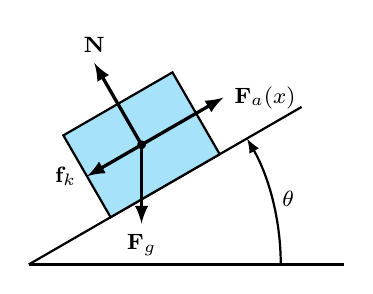
\begin{tikzpicture}[scale=.8]
    \draw[thick] (0,0)--(5,0);
    \draw[axes] (4,0) arc (0:30:4) node[midway,right]{$\theta$};
    \begin{scope}[rotate=30]
      \draw[thick] (0,0)--(5,0);
      \draw[mass] (1.5,0) rectangle (3.5,1.5);
      \fill (2.5,.75) circle (.07);
      \draw[vector] (2.5,.75)--+(1.5,0) node[right]{$\mathbf F_a(x)$};
      \draw[vector] (2.5,.75)--+(0,1.5) node[above]{$\mathbf N$};
      \draw[vector,rotate around={-30:(2.5,.75)}]
      (2.5,.75)--+(0,-1.25) node[below]{$\mathbf F_g$};
      \draw[vector] (2.5,.75)--+(-1,0) node[left]{$\mathbf f_k$};
    \end{scope}
  \end{tikzpicture}
  \caption{Free-body diagram of a crate being pushed up a ramp.}
  \label{example-fbd}
\end{figure}

We can calculate the work done by each of these forces:
\begin{itemize}[topsep=0pt,leftmargin=18pt]
\item The work done by the normal force is zero, because the force is
  perpendicular to the direction of motion, and the dot product is zero:
  \begin{equation*}
    W_N=\int\underbrace{\mathbf N\cdot\dl\mathbf x}_{=0}=0
  \end{equation*}
\item The work done by kinetic friction is negative, because the friction force
  is in the opposite direction to motion, and therefore the dot product gives
  a $-1$.
  \begin{equation*}
    W_f=\int\mathbf F_k\cdot\dl\mathbf x=-\int F_k\dl x=-\mu_k N\Delta x<0
  \end{equation*}
\item The work done by gravity is also negative, $W_g<0$, because the component
  of gravity along the direction of motion is in the opposite direction. (This
  is badly written!!)
\item The work done by the applied force is positive, because applied force is
  in the same direction as motion:
  \begin{equation*}
    W_a(x)=\int_{x_0}^x F_a\dl x>0
  \end{equation*}
\end{itemize}
We can also calculate the total work (i.e.\ the net work) done by summing the
work done by each force:
\begin{equation*}
  W_\text{net}=W_a+W_N+W_g +W_f
  =\int\left(\mathbf F_a+\mathbf N+\mathbf F_g+\mathbf f\right)\cdot\dl\mathbf x
  =\int\mathbf F_\text{net}\cdot\dl\mathbf x
\end{equation*}



\section{Kinetic Energy}
When a net force acts on an object\footnote{We will assume that the mass of the
object is constant.} to accelerate it, we can calculate the total amount of
work done on the object. %(i.e.\ the net work $W_\text{net}$, or the work done
%by the net force $F_\text{net}$).
In one dimension\footnote{When you do this problem ``properly'' in 2D or 3D,
the only difference is the dot product, which only \emph{slightly} increases
the complexity of the problem from the 1D case:
\begin{equation*}
  W_\text{net}
  = \int\mathbf F_\text{net}(\mathbf x)\cdot\dl\mathbf x
  = \cdots = m\int\mathbf v\cdot\dl\mathbf v
\end{equation*}
The difference in the dot product is a lot easier to evaluate than you might
think:
\begin{equation*}
  m\int\mathbf v\cdot\dl\mathbf v
  =m\left(\int v_x\dl v_x + \int v_y\dl v_y + \int v_z\dl v_z\right)
  =\left(\frac12mv_x^2+\frac12mv_y^2 + \frac12mv_z^2\right)
  =\frac12mv^2
\end{equation*}
where $v^2=v_x^2+v_y^2+v_z^2$. This is, of course, the same result that we
got from the one-dimensional case.}, %and assuming that mass is constant,
it is given by:
\begin{equation}
  W_\text{net}
  =\int_{x_0}^{x_1}F_\text{net}(x)\dl x
  =\int ma\dl x
  =m\int\diff vt\dl x
\end{equation}
Since both $v(t)$ and $x(t)$ are continuously differentiable functions in time,
we can switch the order of the differentiation:
\begin{equation*}
  =m\int\diff xt\dl v=m\int_{v_0}^{v_1}v\dl v
\end{equation*}
The limits of integration switch from the initial and final position ($x_0$ and
$x_1$) to the initial and final velocitties, where $v_0=v(x_0)$ and
$v_1=v(x_1)$. Evaluating this integral, we have:
\begin{equation*}
  =m\int_{v_0}^{v_1}v\dl v
  =\frac12mv^2\Big|^{v_1}_{v_0}
  =\frac12mv_1^2-\frac12mv_0^2
  =\Delta K
\end{equation*}
where $K$ is defined as the \textbf{kinetic energy}\footnote{This is more
specifically called the \emph{translational} kinetic energy, and it shoud be
distinguished from the \emph{rotational kinetic energy} which is used when an
object is rotating about a pivot.}:
\begin{equation}
  \boxed{
    K=\frac12mv^2
  }
\end{equation}
The definition of kinetic energy came from this integration: when there is a
net force on the object, and it is doing work, that work is equal to the change
in \emph{something}, and we \emph{define} that as kinetic energy. This is the
\textbf{work-energy theorem}\footnote{Also known as the work-energy principle}:
\begin{equation}
  \boxed{
    W_\text{net}=\Delta K
  }
  \label{work-energy-theorem}
\end{equation}
When there are multiple forces acting on an object, the positive net work
increases the kinetic energy of the object, while negative net work decreases
kinetic energy. Eq.~(\ref{work-energy-theorem}) applies regardless of
\emph{what} the net force is comprised of. Most importantly, this theorem
turns a potentially difficult integration problem (integrating $W_\text{net}$)
into a simple algebraic expression ($\Delta K$).


%  \textbf{Example 1:} A force $F=4x$ (in newtons) acts on an object of mass
%  \SI2{\kilo\gram} as it moves along the $x$-axis from $x=1$ to $x=\SI5\metre$.
%  Given that the object is at rest at $x=1$,
%  \begin{enumerate}[(a)]
%  \item Calculate the net work
%  \item What is the final speed of the object?
%  \end{enumerate}


\section{Potential Energy}

\subsection{Gravitational Force \& Gravitational Potential Energy}
Consider an object that is free-falling under the force of gravity over a
distance of $\Delta x$, shown in Fig.~\ref{falling1}:
\begin{figure}[ht]
  \centering
  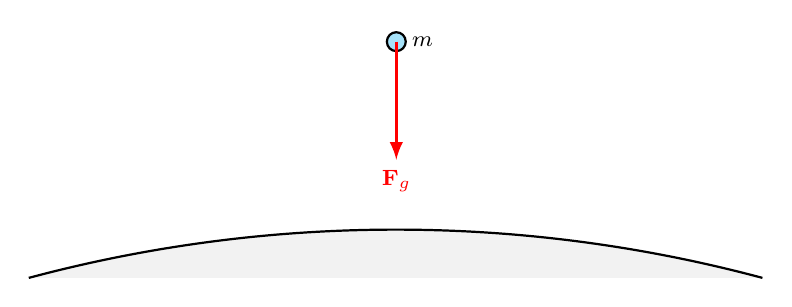
\begin{tikzpicture}[scale=.6]
    \draw[thick,fill=gray!10] (7.75,0) arc (75:105:30);
    \draw[mass] (0,5) circle (.2) node[right=2]{$m$};
    \draw[vector,red] (0,5)--+(0,-2.5) node[below]{$\mathbf F_g$};
  \end{tikzpicture}
  \caption{Gravitational force on a free-falling object.}
  \label{falling1}
\end{figure}
When $\Delta\mathbf x$ is small, $\mathbf g$ can be considered to be constant,
and therefore $\mathbf F_g=m\mathbf g$ is a constant force. Since both the
gravitional force and displacement are in the same direction, the work done by
gravity ($W_g$) is \emph{positive}. From the work-energy theorem
(Eq.~\ref{work-energy-theorem}), there is an increase in kinetic energy, and
the object speeds up, i.e.:
\begin{equation*}
  W_g=mg\Delta x>0 \quad\longrightarrow\quad \Delta K > 0
\end{equation*}
But the work done by gravitational force can also be expressed in terms of the
change in height, shown in Fig.~\ref{falling2}.
\begin{figure}[ht]
  \centering
  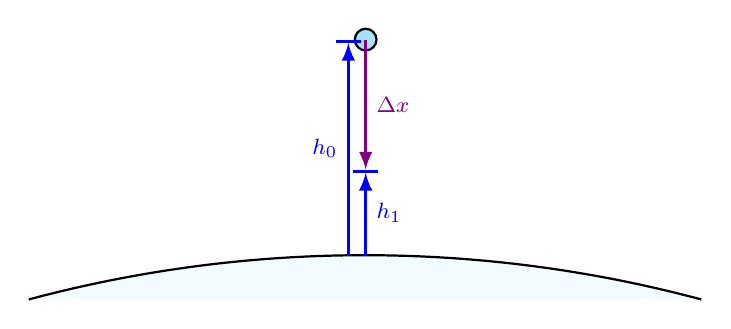
\begin{tikzpicture}[scale=.55]
    \draw[thick,fill=cyan!5] (7.75,0) arc (75:105:30);
    \draw[mass] (0,6) circle (.25);
    \draw[vector,violet] (0,6)--(0,3) node[midway,right]{$\Delta x$};
    \draw[very thick,->|,blue] (-.4,1)--(-.4,6) node[midway,left]{$h_0$};
    \draw[very thick,->|,blue] (0,1)--(0,3) node[midway,right]{$h_1$};
  \end{tikzpicture}
  \caption{Work done by gravity in a uniform gravitational field in terms of
  height above ground}
  \label{falling2}
\end{figure}
Using ground as the reference level (i.e.\ $h=0$), the work done by gravity can
be written as:
\begin{equation*}
  W_g = mg(h_0-h_1)
\end{equation*}
We can further modify this equation:
\begin{equation*}
  W_g= mg(h_0-h_1)=-mg(h_1-h_0)=-(mgh_1-mgh_0) = -\Delta U_g
\end{equation*}
where $U_g$ is defined as the \textbf{gravitational potential energy}:
\begin{equation}
  \boxed{U_g=mgh}
\end{equation}
Since the choice of the reference level is rather arbitrary, we are instead
more interested in the \emph{change} in gravitational potential energy, which
is related to the work done by gravity, i.e.:
\begin{equation}
  \boxed{
    W_g=-\Delta U_g
  }\quad\text{where}\quad
  \boxed{
    \Delta U_g=mg\Delta h
  }
  \label{work-potential-energy}
\end{equation}
In Eq.~\ref{work-potential-energy}, we note some special relationships between
the work done by gravity ($W_g$) and the change in the gravitational potential
energy ($U_g$):

\fcolorbox{black}{yellow!10}{
  \begin{minipage}{.95\textwidth}
    \begin{itemize}[nosep]
    \item \emph{Positive} work by gravity \emph{decreases} gravitational
      potential energy, while
    \item \emph{Negative} work by gravity \emph{increases} gravitational
      potential energy
    \item $W_g$ depends on the end points $h_0$ and $h_1$, but not \emph{how}
      it went from $h_0\rightarrow h_1$
    \item Only work done by $\mathbf F_g$ can affect $U_g$
    \end{itemize}
  \end{minipage}
}

As we look at work done by other forces, we will begin to see the same pattern
emerge for other forces.

\subsection{Spring Force \& Elastic Potential Energy}
The \textbf{spring force} $\mathbf F_s$ is the force that a
compressed/stretched spring exerts on the object connected to it, shown in
Fig.~\ref{hooke1}. An \emph{ideal} spring obeys \textbf{Hooke's law}, which
states that the spring force on a compressed/stretched spring is proportional
to the amount of spring displacement $\mathbf x$, and acts in the opposition
to the diplacement:
\begin{equation}
  \boxed{
    \mathbf F_s=-k\mathbf x
  }
\end{equation}
The constant $k$ is called the \textbf{spring constant}\footnote{The spring
constant is also called the \textbf{force constant}, \textbf{Hooke's constant},
and in many engineering textbooks, \textbf{spring rate}.}, with a unit of
\emph{newton per meter} (\si{\newton\per\metre}). The spring constant depends
on the geometry of the spring, as well as the material that it is made of.
\begin{figure}[ht]
  \centering
  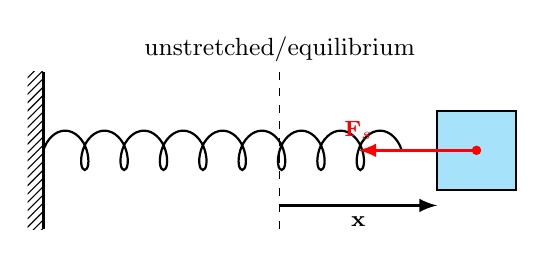
\begin{tikzpicture}
    \draw[mass] (5,.5) rectangle (6,1.5);
    \draw[thick,
      decoration={aspect=.6,segment length=5mm, amplitude=2.5mm, coil},
      decorate] (0,1)--(5,1);
    \fill[pattern=north east lines] (-.2,0) rectangle (0,2);
    \draw[thick] (0,.0)--(0,2);
    \fill[red] (5.5,1) circle (.06);
    \draw[vector,red] (5.5,1)--(4,1) node[above]{$\mathbf F_s$};
    \draw[dashed] (3,0)--(3,2) node[above]{\small unstretched/equilibrium};
    \draw[vector] (3,.3)--(5,.3) node[midway,below]{$\mathbf x$};
  \end{tikzpicture}
  \hspace{.2in}
  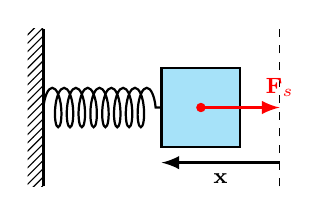
\begin{tikzpicture}
    \fill[pattern=north east lines] (-.2,0) rectangle (0,2);
    \draw[thick] (0,0)--(0,2);
    \draw[dashed] (3,0)--(3,2);
    \draw[mass] (1.5,.5) rectangle (2.5,1.5);
    \draw[thick,decorate,
      decoration={aspect=.3,segment length=1.5mm, amplitude=2.5mm, coil}]
    (0,1)--(1.5,1);
    \draw[vector] (3,.3)--(1.5,.3) node[midway,below]{$\mathbf x$};
    \fill[red] (2,1) circle (.06);
    \draw[vector,red] (2,1)--(3,1) node[above]{$\mathbf F_s$};
  \end{tikzpicture}
  \caption{Direction of spring force is always opposite to spring
    displacement.}
  \label{hooke1}
\end{figure}

As the spring force moves a mass connected to the spring, the work done by
the spring force is:
\begin{equation}
  W_s=\int_{x_0}^{x_1}F_s\dl x =-k\int_{x_0}^{x_1} x\dl x
  =-\frac12kx^2\Big|^{x_1}_{x_0}=-\Delta U_s
\end{equation}
where $U_s$ is now defined as the \textbf{elastic potential energy}:
\begin{equation}
  \boxed{
    U_s=\frac12kx^2
  }
\end{equation}
Therefore, the work done by the spring force is related to the elastic
potential energy by:
\begin{equation}
  \boxed{
    W_s=-\Delta U_s
  }
\end{equation}

\fcolorbox{black}{yellow!10}{
  \begin{minipage}{.95\textwidth}
    \begin{itemize}[nosep]
    \item \emph{Positive} work by the spring \emph{decreases} spring potential
      energy, while
    \item \emph{Negative} work by the spring \emph{increases} spring potential
      energy
    \item $W_s$ depends on the end points $x_0$ and $x_1$, but not \emph{how}
      it went from $x_0$ to $x_1$
    \item Only work done by $\mathbf F_s$ can affect $U_s$
    \end{itemize}
  \end{minipage}
}


\subsection{Electrostatic Force \& Electric Potential Energy}
Similar to the attractive force between masses, there is also a mutually
attractive or repulsive force between charged particles, given by
\textbf{Coulomb's law}:
\begin{equation}
  \boxed{
    \mathbf F_q=\frac{kq_1q_2}{r^2}\hat{\mathbf r}
  }
\end{equation}

The integral is nearly identical to that for the gravitational force:
\begin{equation}
  W_q=\int\mathbf F_q\cdot\dl\mathbf r
  =kq_1q_2\int_{r_0}^{r_1}\frac{\dl r}{r^2}
    =-\frac{kq_1q_2} r\Big|^{r_2}_{r_1}=-\Delta U_q
\end{equation}
where $U_q$ is the \textbf{electric potential energy} that is stored between
the two point charges, defined as:
\begin{equation}
  \boxed{
    U_q = \frac{kq_1q_2}r
  }
\end{equation}

Again, we see the same properties that we have observed 

\fcolorbox{black}{yellow!10}{
  \begin{minipage}{\textwidth}
    \begin{itemize}[nosep]
    \item\emph{Positive} work by the electric force \emph{decreases} electric
      potential energy, while
    \item\emph{Negative} work by the electric force \emph{increases} electric
      potential energy
    \item $W_q$ depends on the end points $r_0$ and $r_1$, but not \emph{how}
      it went from $r_0\rightarrow r_1$
    \item Only work done by $\mathbf F_q$ can affect $U_q$
    \end{itemize}
  \end{minipage}
}


\section{Conservative Forces}

These forces are called \textbf{conservative forces}
\begin{itemize}[nosep]
\item Gravitational force $\mathbf F_g$
\item Spring force $\mathbf F_s$
\item Electrostatic force $\mathbf F_q$
\item Magnetic force $\mathbf F_m$
\item Nuclear forces
\end{itemize}
Because they shared these common properties:
\begin{itemize}[nosep]
\item The work done by these forces relate to a change of a potential energy
  \begin{itemize}[nosep]
  \item Positive work decreases this related potential energy
  \item Negative work increases this related potential energy
  \end{itemize}
\item The work done by a conservative force is \emph{path independent}, in that
  it depends only on end points, but not \emph{how} it gets from one end point
  to the other
\end{itemize}



By the fundamental theorem of calculus, any conservative forces $\mathbf F$
must be the negative gradient of the potential energies:
\begin{equation}
  \mathbf F=-\nabla U=
  -\diffp Ux\hat{\bm\imath}-\diffp Uy\hat{\bm\jmath}-\diffp Uz\hat{\bm k}
\end{equation}
In one-dimension:
\begin{equation}
  F=-\diff Ux
\end{equation}
The direction of a conservative force \emph{always} decreases the potential
energy. (Pay attention to the negative sign. Students often forget it.)



\subsection{Energy Diagrams}
A plot of potential energy ($U$) vs.\ position ($x$) for a conservative force
\begin{figure}[ht]
  \centering
  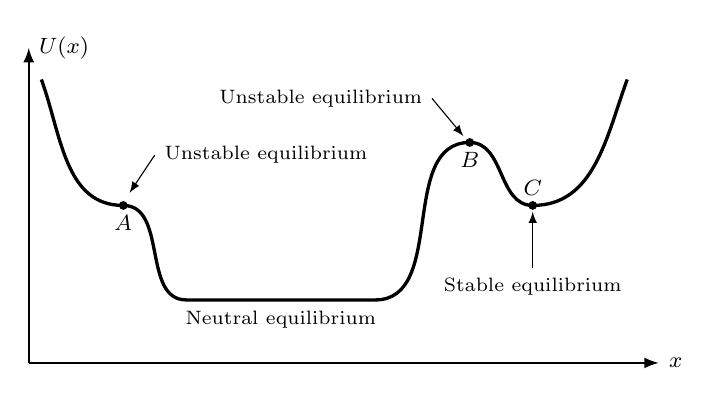
\begin{tikzpicture}[scale=.8]
    \draw[axes] (0,0)--(10,0) node[right]{$x$};
    \draw[axes] (0,0)--(0,5) node[right]{$U(x)$};
    \draw[very thick] (.2,4.5) to[out=-70,in=180](1.5,2.5)
    to[out=0,in=180] (2.5,1)
    --(5.5,1) node[midway,below]{\scriptsize Neutral equilibrium}
    to[out=0,in=180] (7,3.5)
    to[out=0,in=180] (8,2.5)
    to[out=0,in=250] (9.5,4.5);
    \fill(1.5,2.5) circle (.07) node[below]{$A$};
    \fill(7,3.5) circle (.07) node[below]{$B$};
    \fill(8,2.5) circle (.07) node[above]{$C$};
    \draw[<-] (1.6,2.7)--(2,3.3) node[right]{\scriptsize Unstable equilibrium};
    \draw[<-] (6.9,3.6)--(6.4,4.2) node[left]{\scriptsize Unstable equilibrium};
    \draw[<-] (8,2.4)--(8,1.5) node[below]{\scriptsize Stable equilibrium};
  \end{tikzpicture}
\end{figure}

%  The expressions for potential energies also come from integrating the work
%  equation, in that work equals to the change in \emph{something}, and we
%  called that potential energy. Therefore:
%
%  \eq{-.2in}{
%    \boxed{
%      W_c=-\Delta U
%    }
%  }
%  \begin{itemize}
%  \item\vspace{-.15in}$\Delta U$ can be positive or negative depending on the
%    direction of the (conservative) force
%  \item Positive work \emph{decreases} the related potential energy
%  \item Negative work \emph{increases} the related potential energy
%  \end{itemize}

%  Positive work done by conservative forces on an object does two things:
%  \begin{enumerate}[1.]
%  \item Decrease its potential energy, while
%  \item Increase its kinetic energy by the same amount
%  \end{enumerate}
%  Mathematically, this shows that mechanical energy must \emph{always} be
%  conserved when there are only conservative forces:
%
%  \eq{-.1in}{
%    W_c=-\Delta U = \Delta K \quad\longrightarrow\quad
%    \Delta K + \Delta U =0
%  }
%
%  That's why those forces are called conservative forces, and they form the
%  basis for conservation of energy.


\section{Non-Conservative Forces}
%The majority of forces are \textbf{non-conservative}.
The majority of the common forces encountered in introductory physics courses
are generally \textbf{non-conservative}. They include, but not limited to:
\begin{itemize}[nosep]
\item Applied force
\item Tension force
\item Normal force
\item Static friction
\item Kinetic friction
  %\footnote{but sometimes it can also do positive work too.}
\item Aerodynamic lift and drag 
\end{itemize}
The work-energy theorem (Eq.~\ref{work-energy-theorem}) still applies for
non-conservative forces. However, the work done by non-conservative forces
differs from conservative forces in that:
\begin{itemize}
\item There is \textbf{no related potential energies}: the work done by a
  non-conservative force transform energy from one form of kinetic energy to
  another
\item The work is \textbf{path dependent}
\end{itemize}


\subsection{Work by Friction, an Illustration}
We can illustrate the work done by a non-conservative force in general, by
examining how work is done by static friction, using a multi-body problem
commonly studied in dynamics. Two blocks ($m_1$ and $m_2$),
stacked vertically, move to the right without slipping by an external force
$\mathbf F$ applied to $m_1$, as shown in Fig.~\ref{stacked1}. There is a static
coefficient of friction $\mu$ between the two blocks, but the contact between
$m_1$ and the table is frictionless. (The focus of the dynamics study is to
find the maximum acceleration of the blocks, and the maximum $\mathbf F$
without the blocks sliding against each other.) The focus of \emph{this}
example, however, is to find the work done by the forces between the blocks as
they accelerate.
\begin{figure}[ht]
  \centering
  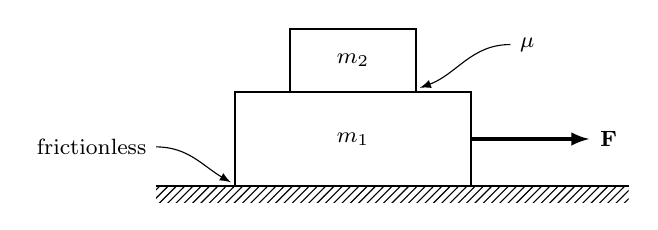
\begin{tikzpicture}
    \fill[pattern=north east lines] rectangle(6,-.2);
    \draw[thick] (0,0)--(6,0);
    \draw[thick] (1,0) rectangle (4,1.2) node[midway]{$m_1$};
    \draw[thick] (1.7,1.2) rectangle (3.3,2) node[midway]{$m_2$};
    \draw[vector] (4,.6)--+(1.5,0) node[right] {$\mathbf F$};
    \draw[<-] (0.95,0.05) to[out=150,in=0] (0,.5) node[left]{frictionless};
    \draw[<-] (3.35,1.25) to[out=20, in=180] (4.5,1.8) node[right]{$\mu$};
  \end{tikzpicture}
  \caption{An external force is applied to move two stacked blocks.}
  \label{stacked1}
\end{figure}

The free-body diagrams of the blocks are shown in Fig.~\ref{stacked-fbd}.
(The forces highlighted in the same colour are action-reaction pairs.) The
static friction between $m_1$ and $m_2$ is $\mathbf f$.
\begin{figure}[ht]
  \centering
  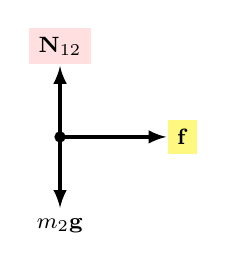
\begin{tikzpicture}[scale=.9]
    \fill circle (.08);
    \draw[vector] (0,0)--(0,-1) node[below]{$m_2\mathbf g$};
    \draw[vector] (0,0)--(0, 1) node[above,fill=pink!50]{$\mathbf N_{12}$};
    \draw[vector] (0,0)--(1.5,0) node[right,fill=yellow!50]{$\mathbf f$};
  \end{tikzpicture}
  \hspace{.2in}
  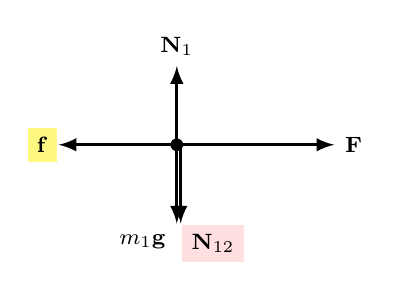
\begin{tikzpicture}
    \fill circle (.08);
    \draw[vector] (0,0)--(0,-1) node[below left]{$m_1\mathbf g$};
    \draw[vector] (.05,0)--(.05,-1)
    node[below right,fill=pink!50]{$\mathbf N_{12}$};
    \draw[vector] (0,0)--(0, 1) node[above]{$\mathbf N_1$};
    \draw[vector] (0,0)--(-1.5,0) node[left,fill=yellow!50]{$\mathbf f$};
    \draw[vector] (0,0)--(2,0) node[right]{$\mathbf F$};
  \end{tikzpicture}
  \caption{Free-body diagrams of the stacked masses.}
  \label{stacked-fbd}
\end{figure}

The top block $m_2$ accelerates to the right because there is static
friction $\mathbf f$ at the interface with $m_1$. Static friction is the
\emph{only} force doing work on $m_2$, and the work done by $\mathbf f$ is
\emph{positive}. $m_2$ gains kinetic energy, consistent with the work-energy
theorem. The change in kinetic energy in $m_2$ as it moves from
$x_0\longrightarrow x_1$ is
\begin{equation*}
  \Delta K_2=\int_{x_0}^{x_1} f\dl x
\end{equation*}
On the bottom block $m_1$, as it moves to the right, applied force $\mathbf F$
does positive work, while static friction $\mathbf f$ does \emph{negative}
work. At a minimum, we conclude that energy is transferred from $m_1$ to $m_2$,
but we can do a more thorough (although still very simple) analysis to find out
how much.

Without friction between $m_1$ and $m_2$, the net force on $m_1$ would have
just been the applied force $\mathbf F$, and the change in kinetic energy after
moving from $x_0\longrightarrow x_1$ to the right would have been simply
\begin{equation*}
  \Delta K_1 = \int_{x_0}^{x_1} F\dl x
\end{equation*}
But with the static friction force present, the gain in kinetic energy is
lowered:
\begin{equation*}
  \Delta K_1 = \int_{x_0}^{x_1} F_\text{net}\dl x =
  \int_{x_0}^{x_1} (F-f)\dl x = \int_{x_0}^{x_1} F\dl x -
  \underbrace{\int_{x_0}^{x_1} f\dl x}_{\Delta K_2}
\end{equation*}
The presence of static friction reduced the kinetic energy of $m_1$ by the
exactly same amount that is gained by $m_2$. We conclude that work done by
friction transfers kinetic energy from one block to another.

\subsection{Work by Kinetic Friction}


\section{Internal/Thermal Energy}

Consider a container of gas of mass $M$ moving at speed $v$ at a height $h$
above Earth (shown in Fig.~\ref{fig:gas}). It has a bulk kinetic energy of
\begin{equation*}
  K=\dfrac12 Mv^2
\end{equation*}
and a gravitational potential energy\footnote{Using the ground level as the
reference} of
\begin{equation*}
  U_g=Mgh
\end{equation*}
But the random motion of the air molecules also contribute to additional
energy, called the \textbf{internal energy} $E_\text{int}$, also known as the
\textbf{thermal energy}.

\begin{figure}[ht]
  \centering
  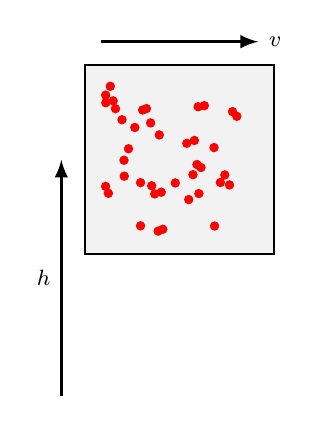
\begin{tikzpicture}
    \draw[thick,fill=gray!10] (-.2,-.2) rectangle (2.2,2.2);
    \draw[vector] (0,2.5)--(2,2.5) node[right]{$v$};
    \draw[vector] (-.5,-2)--(-.5,1) node[midway,left]{$h$};
    \foreach \i in {1,...,40} \fill[red] (rand+1,rand+1) circle (.06);
  \end{tikzpicture}
  \caption{A container of gas moving above Earth has kinetic, gravitational
    potential, as well as internal eneries}
  \label{fig:gas}
\end{figure}
Internal energy of a system of molecules is the sum of all their kinetic and
potential energies at the microscopic level:
\begin{equation*}
  E_\text{int}=K_\text{micro} + U_\text{micro}
\end{equation*}
Internal energy is proportional to molecules' \textbf{absolute temperature},
measured in \emph{kelvin}.\footnote{For those who are keen to know, for a
monatomic or ideal gas, the internal energy comes entirely from the kinetic
energy from the 3 degrees to translational freedom, and is given by
\begin{equation*}
  E_\text{int}=\dfrac32Nk_bT
\end{equation*}
where $N$ is the number of molecules, $k_b$ is the Boltzmann's constant.%, and
%$T$ is the absolute/thermodynamic temperature, which is measured in kelvin.
For a diatomic gas, there are 3 degrees of translational freedom, and 2 degrees
of rotational freedom, and the internal energy is given by:
\begin{equation*}
  E_\text{int}\approx\dfrac52NkT
\end{equation*}
For solids, there are 3 degrees of translational freedom, and 3 degrees of
degrees of vibrational freedom, and therefore the internal energy is:
\begin{equation*}
  E_\text{int}\approx3Nk_bT
\end{equation*}
}
Discussions on thermal/internal energy and the behavior of gases and solids
are part of a much larger discipline within physics called
\textbf{thermodynamics}. We will not be studying thermodynamics in this
booklet.



\section{Conservation of Energy}

The \textbf{law of conservation of energy} states that the change in the total
energy of a system $E_\text{sys}$ is equal to the net external work
$W_\text{ext}$ done to it.
\begin{equation}
  \boxed{
    \Delta E_\text{sys}=W_\text{ext}
  }
  \label{conservationlaw}
\end{equation}
Where the system energy include both the bulk kinetic energies and potential
energies (collectively known as the \textbf{mechanical energy}), as well as the
internal (or thermal) energy:
\begin{equation}
  E_\text{sys}=\underbrace{\sum K + \sum U}_\text{mechanical energy}+E_\text{int}
  \label{law1}
\end{equation}
Substitutiting the expression from Eq.~(\ref{law1}) into
(\ref{conservationlaw}), we get:
\begin{equation}
  \boxed{
    \Delta K + \Delta U + \Delta E_\text{int} = W_\text{ext}
  }
\end{equation}
In an isolated system that does not interact with the outside (and therefore
no external work can be done), conservation of energy reduces to
\begin{equation}
  \Delta K + \Delta U + \Delta E_\text{int} = 0
\end{equation}

%  In almost all of the problem encountered in AP Physics C, there will be no
%  change in the internal energy of the system, and conservation of energy
%  reduces to:
%  
%  \eq{-.1in}{
%    \boxed{ \Delta K + \Delta U = W_\text{ext} }\quad\rightarrow\quad
%    \boxed{ U_1 + K_1 + W_\text{ext} = U_2 + K_2 }
%  }
%
%  External work $W_\text{ext}$ is
%  \begin{itemize}
%  \item\textbf{Positive} if work is done \text{to} the system
%  \item\textbf{Negative} if work is done \text{by} by the system to the
%    surrounding
%  \end{itemize}

%  An \textbf{isolated system} is a system of objects that does not interact with
%  the surrounding. Think of an isolated system as a bunch of objects inside an
%  insulated box.
%  \begin{center}
%    \begin{tikzpicture}[scale=.7]
%      \fill[pattern=north east lines] rectangle(5,4);
%      \draw[thick] rectangle(5,4);
%      \draw[thick,fill=blue!5](.2,.2) rectangle(4.8,3.8);
%      \draw[thick,
%        decoration={aspect=.3,segment length=2mm, amplitude=2.5mm, coil},
%        decorate] (2.5,3.8)--(2.5,2.2) node[midway,right]{$\;\;k$};
%      \draw[thick,fill=cyan](2,2.25) rectangle(3,1.25) node[midway]{$m$};
%    \end{tikzpicture}
%  \end{center}
%  Since the system is isolated from the surrounding environment, the
%  environment can't do any work on it. Likewise, the energy inside the system
%  cannot escape either.


\subsection{Gravity}
Assuming that there are no friction and drag (air resistance), a free-falling
object (Fig.~\ref{fig:earth}) forms an isolated system with Earth. 
\begin{figure}[ht]
  \centering
  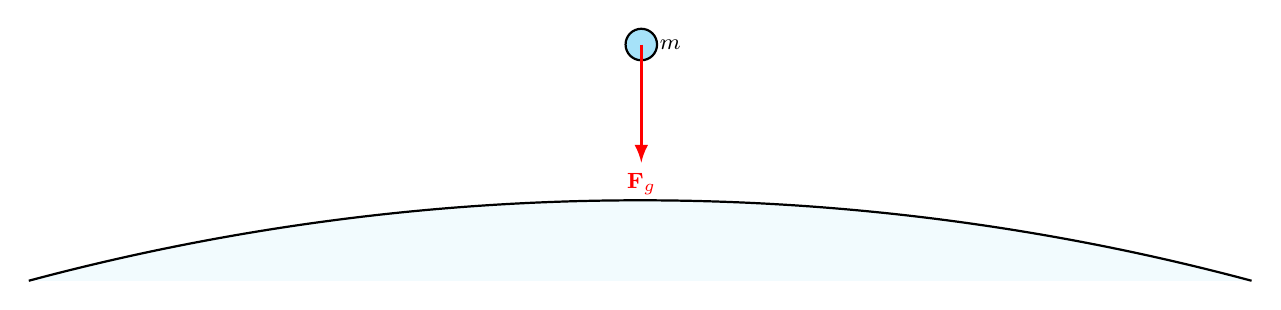
\begin{tikzpicture}
    \draw[thick,fill=cyan!5] (7.75,0) arc (75:105:30);
    \draw[mass] (0,3) circle (.2) node[right=3]{$m$};
    \draw[vector,red] (0,3)--(0,1.5) node[below]{$\mathbf F_g$};
  \end{tikzpicture}
  \caption{Isolated system with a mass and Earth}
  \label{fig:earth}
\end{figure}
This isolated system consists only of Earth and the mass $m$, and the energy of
the system is the kinetic energy of the mass ($K$) and the gravitational
potential energy stored between the the mass and Earth ($U_g$). Beginning with
the work-energy theorem, we recognize that as the object falls, the only force
that does work is gravity. And since gravity is conservative, we can also
relate $W_g=-\Delta U_g$.
\begin{align*}
  W_\text{net} &=\Delta K\\
  -\Delta U_g &=\Delta K
\end{align*}
Giving us:
\begin{equation}
  \boxed{
    \Delta K + \Delta U_g=0
  }
  \quad\text{or}\quad
  \boxed{
    K+U_g=\text{constant}
  }
\end{equation}
The sum of the system's kinetic energy and gravitational potential is constant.

\subsection{Horizontal Spring-Mass System}
Assuming that there are no friction, drag or other damping forces present, a
horizontal spring-mass system is an isolated system.
\begin{figure}[ht]
  \centering
  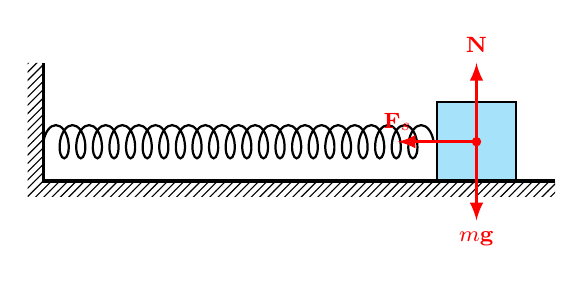
\begin{tikzpicture}
    \draw[mass] (5,.5) rectangle (6,1.5);
    \draw[thick,decorate,
      decoration={coil,amplitude=6,aspect=.5,segment length=6}] (0,1)--(5,1);
    \fill[pattern=north east lines] (6.5,.5)--(6.5,.3)--(-.2,.3)
    --(-.2,2)--(0,2)--(0,.5)--cycle;
    \draw[very thick] (0,2)--(0,.5)--(6.5,.5);
    \draw[vector,red] (5.5,1)--(5.5,0) node[below]{$m\mathbf g$};
    \draw[vector,red] (5.5,1)--(5.5,2) node[above]{$\mathbf N$};
    \draw[vector,red] (5.5,1)--(4.5,1) node[above]{$\mathbf F_s$};
    \fill[red] (5.5,1) circle (.06);
  \end{tikzpicture}
\end{figure}
The sum of the kinetic energy of the mass ($K$) and the elastic potential
energy stored in the spring ($U_s$) is constant
\begin{equation}
  K+U_s=\text{constant}
\end{equation}



\subsection{Vertical Spring-Mass System}
Assuming that there are no friction, drag or other damping forces in the
spring, the vertical spring-mass system (consists of the mass, the spring
and Earth) is a closed system.
\begin{figure}[ht]
  \centering
  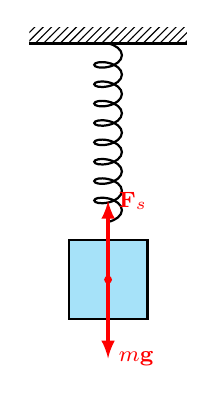
\begin{tikzpicture}
    \draw[mass] (.5,1.5) rectangle(1.5,2.5);% node[midway]{$m$};
    \draw[thick,decorate,decoration={
        aspect=.5,segment length=7, amplitude=5,coil}] (1,5)--(1,2.5); 
    \fill[pattern=north east lines] (0,5) rectangle (2,5.2);
    \draw[very thick] (0,5)--(2,5);
    \draw[vector,red] (1,2)--(1,1) node[right]{$m\mathbf g$};
    \draw[vector,red] (1,2)--(1,3) node[right]{$\mathbf F_s$};
    \fill[red] (1,2) circle (.05);
  \end{tikzpicture}
\end{figure}
The sum of the kinetic energy of the mass ($K$), the gravitational potential
energy stored between the mass and Earth ($U_g$), and the elastic potential
energy stored in the spring ($U_s$) is constant.
\begin{equation}
  K + U_g + U_s=\text{constant}
\end{equation}



\subsection{Simple Pendulum}
Assuming that there are no friction, drag or other damping forces in the
spring, the simple pendulum system (consists of the mass and Earth) is a
closed system.
%    \begin{itemize}
%    \item Gravity ($m\mathbf g$), which is conservative, is the only force that
%      does work
%    \item Tension ($\mathbf T$), which is non-conservative, does not do work on the
%      pendulum because it is always perpendicular to the motion of the pendulum
%      bob
%    \end{itemize}
%    The sum of the kinetic energy of the mass ($K$), the gravitational
%    potential energy stored between the mass and Earth ($U_g$) is constant:
%
%    \eq{-.2in}{
%      K + U_g =\text{constant}
%    }
    
\begin{figure}[ht]
  \centering
  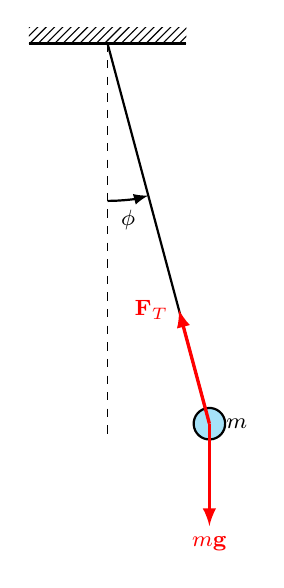
\begin{tikzpicture}
    \fill[pattern=north east lines] (-1,0) rectangle (1,0.2);
    \draw[thick] (-1,0)--(1,0);
    \begin{scope}[rotate=15]
      \draw[thick] (0,0)--(0,-5);
      \draw[mass] (0,-5) circle (.2) node[right]{$\;m$};
      \draw[red,vector] (0,-5)--(0,-3.5) node[left]{$\mathbf F_T$};
      \draw[red,vector,rotate around={-15:(0,-5)}] (0,-5)--(0,-6.3)
      node[below]{$m\mathbf g$};
    \end{scope}
    \draw[dashed,thin] (0,0)--(0,-5);
    \draw[axes] (0,-2) arc (270:285:2) node[midway,below]{$\phi$};
  \end{tikzpicture}
\end{figure}



\subsection{Isolated System with Changing Internal Energy}

Energy is always conserved as long as your system is defined properly. In
this case, the system consists of a mass, a spring, Earth and all the air
molecules inside the box:
\begin{figure}[ht]
  \centering
  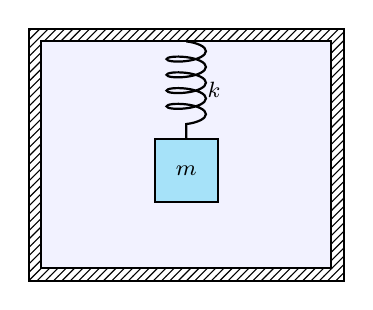
\begin{tikzpicture}[scale=.8,thick]
    \fill[pattern=north east lines] rectangle (5,4);
    \draw rectangle (5,4);
    \draw[fill=blue!5] (.2,.2) rectangle (4.8,3.8);
    \draw[thick,decorate,
      decoration={aspect=.3,segment length=2mm, amplitude=2.5mm, coil}]
    (2.5,3.8)--(2.5,2.25) node[midway,right=4]{$k$};
    \draw[mass] (2,2.25) rectangle(3,1.25) node[midway]{$m$};
  \end{tikzpicture}
\end{figure}
The energies of this system include
\begin{itemize}
\item Kinetic energy of the mass ($K$)
\item Gravitational potential energy ($U_g$) between the mass and Earth
\item Elastic potential energy ($U_s$) stored in the spring
  \item Internal energy ($E_\text{int}$) of the air molecules
\end{itemize}

As the mass vibrates, friction and drag with air slows it down, converting the
kinetic energy of the mass into the internal energy of the air. Total energy
is conserved even as the mass stops moving

\begin{figure}[ht]
  \centering
  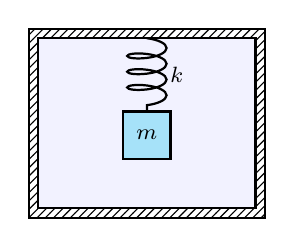
\begin{tikzpicture}[scale=.6]
    \fill[pattern=north east lines] rectangle(5,4);
    \draw[thick] rectangle(5,4);
    \draw[thick,fill=blue!5] (.2,.2) rectangle(4.8,3.8);
    \draw[thick,
      decoration={aspect=.3,segment length=2mm, amplitude=2.5mm, coil},
      decorate] (2.5,3.8)--(2.5,2.25) node[midway,right]{$\;\;k$};
    \draw[mass] (2,2.25) rectangle(3,1.25) node[midway]{$m$};
  \end{tikzpicture}
\end{figure}

\begin{equation}
  K + E_\text{int}+U_g+U_s=\text{constant}
\end{equation}

%  \vspace{.2in}Non-conservative forces doing work are \emph{internal} to the
%  system, and therefore energy is still conserved. (Work done by friction
%  transform from the kinetic energy of the mass to the kinetic energy of the
%  air molecules.)


\section{Isolated System vs.\ Open System}
Accounting for the change in the internal energy of the air molecules is not
always practical, especially when the air molecules are not confined to a box.
\begin{figure}[ht]
  \centering
  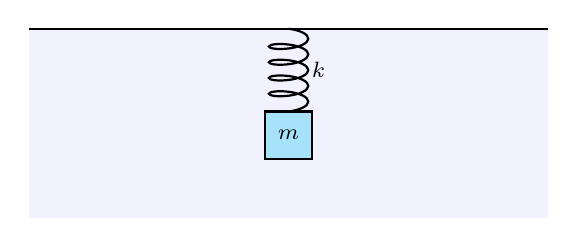
\begin{tikzpicture}[scale=.6,thick]
    \fill[blue!5] (-3,0) rectangle (8,4);
    \draw (-3,4)--(8,4);
    \draw[
      decoration={aspect=.3,segment length=2mm, amplitude=2.5mm, coil},
      decorate] (2.5,4)--(2.5,2.25) node[midway,right]{$\;\;k$};
    \draw[mass] (2,2.25) rectangle (3,1.25) node[midway]{$m$};
  \end{tikzpicture}
\end{figure}
The solution:
\begin{itemize}
\item Take the air molecule out of the \emph{system}
\item No longer an isolated system
\item Treat the negative work done by kinetic friction and drag as
  \emph{external work} between initial (1) and final (2) states
  
  \begin{equation}
    K_1 + U_{g1} + U_{e1} + W_f= K_2 + U_{g2} + U_{e2}
  \end{equation}
\end{itemize}

%  If \emph{only} conservative forces are doing work, mechanical energy (i.e.\
%  $K+U$) is always conserved:
%
%  \eq{-.2in}{
%    \boxed{K+U =K'+U'}
%  }
%  
%  When external non-conservative forces are also doing work, instead of
%  \emph{trying} to isolate the system, we can instead calculate the work done
%  by them $W_{nc}$ and add it to the total energy of the system
%    
%  \eq{-.2in}{
%    \boxed{K+U+W_{nc}=K'+U'}
%  }
%
%
%
%\textbf{Example:} A mass $m$ is dropped from a height of $h$ above the
%equilibrium position of a spring. Set up the equation that determines the
%spring's compression $d$ when the object is instantaneously at rest.
%\begin{center}
%  \pic{.35}{spring-example1}
%\end{center}
%
%
%  \textbf{Example 3:} A mass $m$ is pulled a distance $d$ up an incline (angle
%  of elevation $\theta$) at constant speed using a rope that is parallel to
%  the incline. The coefficient of friction is $\mu_k$.
%  \begin{enumerate}[(a)]
%  \item What is the magnitude of the tension force in the rope?
%  \item What is the magnitude of the normal force?
%  \item What is the work done by the normal force?
%  \item What is the work done by friction?
%  \item What is the work done by the tension force?
%  \item What is the net work?
%  \item What is the change in total mechanical energy?
%  \item Show that $\Delta E_{mech}=W_{nc}$.
%  \end{enumerate}
%
%
%
%\section{Power \& Efficiency}
%
%\textbf{Power} is the \emph{rate} at which work is done, i.e.\ the rate at
%which energy is being transformed:
%
%\begin{equation}
%  \boxed{P(t) = \diff Wt}\quad\quad
%  \boxed{\overline P = \frac W{\Delta t}}
%\end{equation}
%\begin{center}
%  \begin{tabular}{l|c|c}
%    \rowcolor{pink}
%    \textbf{Quantity}  & \textbf{Symbol} & \textbf{SI Unit} \\ \hline
%    Instantaneous and average power & $P$, $\overline P$ & \si\watt \\
%    Work done          & $W$ & \si\joule \\
%    Time interval      & $\Delta t$ & \si\second
%  \end{tabular}
%\end{center}
%In engineering, power is often more critical than the actual amount of work
%done.
%
%
%If a constant force is used to push an object at a constant velocity, the
%power produced by the force is:
%  
%\begin{equation}
%  P=\diff Wt=\frac{\mathbf F\cdot\dl\mathbf x}{\dl t}
%  =\mathbf F\cdot\diff{\mathbf x}t
%  \quad\rightarrow\quad
%  \boxed{P=\mathbf F\cdot\mathbf v}
%\end{equation}
%    
%Application: aerodynamics
%\begin{itemize}
%\item When an object moves through air, the applied force must overcome air
%  resistance (drag force), which is proportional with $v^2$
%\item Therefore ``aerodynamic power'' must scale with $v^3$ (i.e.\ doubling
%  your speed requires $2^3=8$ times more power)
%\item Important when aerodynamic forces dominate
%\end{itemize}
%
%\textbf{Efficiency} is the ratio of useful energy or work output to the total
%energy or work input
%
%\begin{equation}
%  \boxed{ \eta = \frac{E_o}{E_i}\times\SI{100}\percent }\quad
%  \boxed{ \eta = \frac{W_o}{W_i}\times\SI{100}\percent }
%\end{equation}
%\begin{center}
%  \begin{tabular}{l|c|c}
%    \rowcolor{pink}
%    \textbf{Quantity} & \textbf{Symbol} & \textbf{SI Unit} \\ \hline
%    Useful output energy & $E_o$  & \si\joule \\
%    Input energy         & $E_i$  & \si\joule \\
%    Useful output work   & $W_o$  & \si\joule \\
%    Input work           & $W_i$  & \si\joule \\
%    Efficiency           & $\eta$ & no units
%  \end{tabular}
%\end{center}
%Efficiency is always $0\leq\eta<\SI{100}\percent$
\end{document}
